%&pdflatex
\documentclass[a4paper,12pt]{article}
\usepackage{amssymb, amsmath}
\usepackage[utf8]{inputenc}
\usepackage[T2A,T1]{fontenc}
\usepackage[english,russian]{babel}
\usepackage{csquotes}
% \IfFileExists{literat.sty}{\usepackage{literat}}{}

\usepackage{fullpage}
\usepackage{indentfirst}
\usepackage[font=small,labelfont=bf,labelsep=period]{caption}
\usepackage{comment}

\usepackage{graphicx}
\usepackage{wrapfig}
\usepackage[skip=0pt]{subcaption}

\newcommand{\Kn}{\mathrm{Kn}}
\newcommand{\NS}{N\!S}
\newcommand{\dd}{\mathrm{d}}
\newcommand{\der}[2][]{\frac{\dd#1}{\dd#2}}
\newcommand{\pder}[2][]{\frac{\partial#1}{\partial#2}}
\newcommand{\pderdual}[2][]{\frac{\partial^2#1}{\partial#2^2}}
\newcommand{\pderder}[3][]{\frac{\partial^2#1}{\partial#2\partial#3}}
\newcommand{\Pder}[2][]{\partial#1/\partial#2}

\usepackage[
    pdfauthor={Rogozin Oleg},
    pdftitle={Numerical analysis of the nonlinear plane Couette flow for hard-sphere molecules},
    colorlinks, pdftex, unicode
]{hyperref}
\usepackage{cleveref}

\usepackage[
    backend=biber,
    hyperref=true,
    autolang=other,                 % multi-language
    mincrossrefs=100,               % to prevent implicit inserts into bibliography
    maxnames=100,                   % print all authors
    style=gost-numeric,
    movenames=false,                % only for biblatex-gost
    sorting=none,
    doi=false,
    isbn=false
]{biblatex}
\bibliography{couette}

\usepackage[toc]{appendix}
\renewcommand{\appendixtocname}{Приложения}
\renewcommand{\appendixpagename}{Приложения}
\renewcommand{\appendixname}{Приложениe}

\title{Численный анализ нелинейного течения Куэтта между двумя параллельными пластинами для газа твёрдых сфер}
\author{Рогозин Олег}

\begin{document}
\maketitle
\tableofcontents

\section{Аннотация}

В широком диапазоне чисел Кнудсена изучено плоское ламинарное течение Куэтта для одноатомного газа твёрдых сфер.
Основное внимание уделено нелинейной задаче и нахождению соответствующих профилей распределения макроскопических величин.
В частности, при конечных числах Маха наблюдается выраженная анизотропия функции распределения,
а следовательно и тензора давления. Этот результат не может быть получен из уравнений Навье"--~Стокса также,
как продольный тепловой поток.
В работе применяются как асимптотические методы для малых чисел Кнудсена (разложение Гильберта),
так и численные методы статистического моделирования (DSMC),
а также непосредственно конечно-разностное решение уравнения Больцмана (метод Черемисина).

\section{Постановка задачи и основные уравнения}

Рассмотрим одноатомный идеальный газ между двумя бесконечными параллельными пластинами с полным диффузным отражением.
Ось абсцисс направлена параллельно пластинам, расстояние между которыми равно \(L\).
В качестве молекулярного потенциала взаимодействия выберем модель твердых сфер.

Течение Куэтта образуется при относительном движении пластин друг относительно друга с продольной скоростью
вдоль оси абсцисс, при этом температура стенок одинакова и остаётся постоянной.
Задача переноса тепла ставится для фиксированного отношения температур покоящихся пластин.

В работе будем иметь дело с безразмерными величинами, такими, что макроскопические величины будут
иметь следующий вид: давление \(pp^{(0)}\), температура \(TT^{(0)}\), плотность \(\rho p^{(0)}/RT^{(0)}\)
скорость \(v_i(2RT^{(0)})^{1/2}\) и тепловой поток \(q_ip^{(0)}(2RT^{(0)})^{1/2}\),
где \(R = k_B/m\) "--- удельная газовая постоянная,
равная отношению постоянной Больцмана \(k_B\) к молекулярной массе \(m\),
а \(T^{(0)}\) "--- средняя температура пластин.
За единицу длины примем расстояние между пластинами \(L\).
Расчётная область, представленная на рис.~\ref{fig:geometry} серым фоном,
лежит в диапазоне \(0 \le y\le 1/2\) вследствие антисимметрии задачи.
Температура и скорость верхней пластины (\(y=1/2\)) равны \((1+\Delta{T}/2)T^{(0)}\)
и \((\Delta{v}/2)(2RT^{(0)})^{1/2}\), соответственно.

\begin{figure}[ht]
    \centering
    \includegraphics{tikz/geometry}
    \caption{Геометрия задачи}
    \label{fig:geometry}
\end{figure}

Стационарное уравнение Больцмана в безразмерных переменных принимает следующий вид:
\begin{equation}\label{eq:Boltzmann}
    \zeta_i\pder[f]{x_i} = \frac1k J(f,f),
\end{equation}
в котором интеграл столкновений
\begin{equation}
    J(f,g) = \frac12 \int (f'g'_* + f'_*g' - fg_* - f_*g) B
    \dd \Omega(\boldsymbol{\alpha}) \boldsymbol{\dd \zeta_*},
\end{equation}
берётся от функции распределения \(f(x_i,\zeta_i)(2p^{(0)})/(2RT^{(0)})^{5/2}\), представленной
в пространстве \((x_iL, \zeta_i(2RT^{(0)})^{1/2})\).
\(\dd \Omega(\boldsymbol{\alpha})\) "--- элемент телесного угла в направлении единичного вектора \(\alpha_i\),
определяющего направление разлётных скоростей:
\[
    \zeta'_i = \zeta_i + \alpha_i\alpha_j(\zeta_{j*}-\zeta_j), \quad
    \zeta'_{i*} = \zeta_{i*} - \alpha_i\alpha_j(\zeta_{j*}-\zeta_j).
\]
Ядро \(B(\alpha_i(\zeta_{i*}-\zeta_i)|,|\zeta_{i*}-\zeta_i|)\)
определяется законом межмолекулярного взаимодействия.
В частном случае модели твёрдых сфер
\begin{equation}
    B = \frac{|\alpha_i(\zeta_{i*}-\zeta_i)|}{4\sqrt{2\pi}}.
\end{equation}
В уравнении~\eqref{eq:Boltzmann} используется модифицированное число Кнудсена
\begin{equation}
    k = \frac{\sqrt\pi}2 \Kn = \frac{\sqrt\pi\ell_0}{2L} =
    \frac{mRT^{(0)}}{2\sqrt{2\pi} d_m^2p^{(0)}L},
\end{equation}
где \(\ell_0\) "--- средняя длина свободного пробега, определяемая радиусом межмолекулярного
взаимодействия \(d_m\) (для модели твёрдых сфер совпадает с диаметром молекулы).

Макроскопические переменные вычисляются с помощью интегрирования функции распределения по формулам:
\begin{alignat*}{2}
    \rho &= \int f \boldsymbol{\dd\zeta}, \\
    v_i &= \frac1{\rho} \int \zeta_i f \boldsymbol{\dd\zeta}, \\
    T &= \frac{2}{3\rho}\int(\zeta_i-v_i)^2 f \boldsymbol{\dd\zeta}, \\
    p_{ij} &= 2 \int(\zeta_i-v_i)(\zeta_j-v_j) f \boldsymbol{\dd\zeta},
        \quad p \equiv p_{ii}/3 = \rho T, \\
    q_i &= \int(\zeta_i-v_i)(\zeta_j-v_j)^2 f \boldsymbol{\dd\zeta}.
\end{alignat*}

\subsection{Линеаризация задачи}
\newcommand{\edzeta}{E\boldsymbol{\dd\zeta}}

Линеаризованное уравнение Больцмана
\begin{equation}\label{eq:linear_Boltzmann}
    \zeta_i \pder[\phi]{x_i} = \frac1k \mathcal{L}(\phi),
\end{equation}
с линеаризованным оператором столкновения
\begin{equation}\label{eq:linear_ci}
    \mathcal{L}(\phi) = \int E_*(\phi'+\phi'_*-\phi-\phi_*) B
    \dd \Omega(\boldsymbol{\alpha}) \boldsymbol{\dd \zeta_*}
\end{equation}
справедливо для слабо возмущённого решения
\begin{equation}\label{eq:linear_condition}
    \phi = \frac{f}{E} - 1 \ll 1, \quad E(\zeta) = \frac1{\pi^{3/2}}\exp\left(\zeta^2\right).
\end{equation}
Cлабо возмущённое локальное максвелловское распределение
\begin{equation}\label{eq:linear_maxwellian}
    \phi_e = \omega + 2\zeta_i v_i + \left(\zeta_i^2-\frac32\right)\tau
\end{equation}
удобно выражается через соответствующие макроскопические величины:
\begin{equation}
    \omega = \rho-1, \quad \tau = T-1, \quad P_{ij} = p_{ij} - \delta_{ij}.
\end{equation}

Задача о газе между двумя параллельными пластинами линеаризуется,
когда на внешние параметры наложены следующие условия:
\begin{equation}\label{eq:weak_perturbation}
    \Delta{v}\ll 1, \quad \Delta{T}\ll 1,
\end{equation}
при этом функция распределения допускает расщепление
\begin{equation}\label{eq:linear_solution}
    \phi = \Delta{v} \zeta_x \Phi_C(y,\zeta_y,\zeta) + \Delta{T} \Phi_H(y,\zeta_y,\zeta),
    \quad \zeta = (\zeta_i^2)^{1/2},
\end{equation}
на задачи течения Куэтта (\(\Phi_C\)) и переноса тепла (\(\Phi_H\)):
\begin{equation}\label{eq:linear_equations}
    \zeta_y \pder[\Phi_C]{y} = \frac1{k\zeta_x}\mathcal{L}(\zeta_x\Phi_C), \quad
    \zeta_y \pder[\Phi_H]{y} = \frac1{k}\mathcal{L}(\Phi_H),
\end{equation}
с граничными условиями на верхней пластине
\begin{equation}\label{eq:linear_bc1}
    \Phi_C^- \left(\frac12,\zeta_y,\zeta\right) = 1, \quad
    \Phi_H^- \left(\frac12,\zeta_y,\zeta\right) = 2\sqrt\pi\int_{\zeta_y>0}\zeta_y\Phi_H^+ \edzeta + \frac{\zeta^2}2-1, \quad
    \zeta_y < 0
\end{equation}
и плоскости антисимметрии
\begin{equation}\label{eq:linear_bc2}
    \Phi_C^+ (0,\zeta_y,\zeta) = -\Phi_C^- (0,-\zeta_y,\zeta), \quad
    \Phi_H^+ (0,\zeta_y,\zeta) = -\Phi_H^- (0,-\zeta_y,\zeta).
\end{equation}
При этом мы ввели следующие обозначения:
\begin{equation}\label{eq:linear_pm_phi}
    \Phi_C^\pm \equiv \Phi_C (\zeta_y \gtrless 0), \quad
    \Phi_H^\pm \equiv \Phi_H (\zeta_y \gtrless 0).
\end{equation}

В итоге макроскопические величины выражаются следующим образом:
\begin{gather*}
    \frac{\omega_{H}}{\Delta{T}} = \int \Phi_H \edzeta, \quad
    \frac{v_{xC}}{\Delta{v}} = \int \zeta_x^2 \Phi_C \edzeta, \quad
    \frac{\tau_{H}}{\Delta{T}} = \int \left(\frac23\zeta^2-1\right) \Phi_H \edzeta, \\
    \frac{P_{xxH}}{\Delta{T}} = 2\int \zeta_x^2 \Phi_H \edzeta, \quad
    \frac{P_{yyH}}{\Delta{T}} = 2\int \zeta_y^2 \Phi_H \edzeta, \quad
    \frac{P_{xyC}}{\Delta{v}} = 2\int \zeta_x^2 \zeta_y \Phi_C \edzeta, \\
    \frac{q_{xC}}{\Delta{v}} = \int \zeta_x^2 \zeta^2 \Phi_C \edzeta - \frac52 \frac{v_{xC}}{\Delta{v}}, \quad
    \frac{q_{yH}}{\Delta{T}} = \int \zeta_y \zeta^2 \Phi_H \edzeta.
\end{gather*}

\section{Методы решения линейной задачи}

\subsection{Свободномолекулярное решение}

Бесстолкновительное линеаризованное уравнение Больцмана
\begin{equation}\label{eq:linear_free}
    \zeta_i \pder[\phi]{x_i} = 0
\end{equation}
для течения Куэтта и переноса тепла имеет простое решение
в виде двухстороннего максвелловского распределения
\begin{equation}\label{eq:linear_free_solution}
    \Phi_C^\pm = \mp 1, \quad
    \Phi_H^\pm = \mp \left(\frac{\zeta^2}{2}-1\right),
\end{equation}
которое даёт следующие значения макроскопических величин:
\begin{gather}\label{eq:linear_free_macro}
    \omega_{H} = \tau_{H} = 0, \quad
    v_{xC} = q_{xC} = 0, \quad
    P_{xxH} = P_{yyH} = 0, \notag \\
    \frac{P_{xyC}}{\Delta{v}} = -\frac1{\sqrt\pi}, \quad
    \frac{q_{yH}}{\Delta{T}} = -\frac1{\sqrt\pi}.
\end{gather}

\subsection{Разложение Грэда"--~Гильберта для малых чисел Кнудсена}

При малых \(k\) имеет место асимптотическое решение~\cite{Sone2007}:
\begin{equation}\label{eq:small_solution}
    \Phi_C = \frac{2y - \zeta_y \mathcal{B}(\zeta) k}{1-2k_0k}, \quad
    \Phi_H = \frac1{1+2d_1k}\left[ \left(\zeta^2-\frac52\right)y
        - \zeta_y \mathcal{A}(\zeta)k \right],
\end{equation}
в котором использованы специальные функции \( \mathcal{A}(\zeta) \) и \( \mathcal{B}(\zeta) \),
определяемые через интегральные уравнения для отдельно взятого молекулярного потенциала:
\begin{gather}
    \mathcal{L}[\zeta_i \mathcal{A}(\zeta)] = -\zeta_i \left( \zeta^2 - \frac52 \right),
    \quad \int_0^\infty \zeta^4 \mathcal{A}(\zeta)E\dd\zeta = 0, \label{eq:def_A} \\
    \mathcal{L}\left[\left(\zeta_i\zeta_j-\frac{\zeta^2}3\delta_{ij}\right) \mathcal{B}(\zeta)\right]
        = -2 \left(\zeta_i\zeta_j-\frac{\zeta^2}3\delta_{ij}\right). \label{eq:def_B}
\end{gather}
Решение~\eqref{eq:small_solution} не удовлетворяет граничным условиям~\eqref{eq:linear_bc1},
поэтому дополнительно корректируется в кнудсеновском слое,
что приводит к следующим значениям макроскопических величин:
\begin{equation}\label{eq:small_macro}
    \begin{gathered}
    \frac{\omega_{H}}{\Delta{T}} = \frac{-y + (\Omega_1^--\Omega_1^+)k}{1+2d_1k}, \quad
    \frac{\tau_{H}}{\Delta{T}} = \frac{y + (\Theta_1^--\Theta_1^+)k}{1+2d_1k}, \\
    \frac{v_{xC}}{\Delta{v}} = \frac{y - (Y_0^--Y_0^+)k}{1-2k_0k}, \\
    \frac{P_{xxH}}{\Delta{T}} = \frac{P_{yyH}}{\Delta{T}} = \frac{\omega_{H}+\tau_{H}}{3\Delta{T}}, \quad
    \frac{P_{xyC}}{\Delta{v}} = - \frac{\gamma_1 k}{1-2k_0k}, \\
    \frac{q_{xC}}{\Delta{v}} = \frac{(H_A^--H_A^+)k}{1-2k_0k}, \quad
    \frac{q_{yH}}{\Delta{T}} = - \frac{5\gamma_2}4 \frac{k}{1+2d_1k}.
    \end{gathered}
\end{equation}
где определены транспортные коэффициенты
\begin{equation}\label{eq:transport_coeffs}
    \gamma_1 = \frac{8\pi}{15}\int_0^\infty \zeta^6 \mathcal{B}(\zeta)E\dd\zeta, \quad
    \gamma_2 = \frac{16\pi}{15}\int_0^\infty \zeta^6 \mathcal{A}(\zeta)E\dd\zeta,
\end{equation}
и коэффициенты скольжения \(k_0\), \(d_1\), а также функции кнудсеновского слоя
\(\Omega_1(\eta)\), \(\Theta_1(\eta)\), \(Y_0(\eta)\), \(H_A(\eta)\),
убывающие экспоненциально [\(=\mathcal{O}(e^{-\eta})\)].
Кроме того,
\begin{equation}\label{eq:def_eta}
     \eta_\pm = \frac{1 \mp 2y}{2k}.
\end{equation}
Приведённые коэффициенты и функции для кинетической модели БКВ и газа твёрдых сфер
подробно табулированы в~\cite{Sone2007}. В частности,
\begin{gather}
    \gamma_1 = 1.270042427, \quad \gamma_2 = 1.922284066, \label{eq:gamma12_coefficients}\\
    k_0 = -1.2540, \quad d_1 = 2.4001. \label{eq:slip_coefficients}
\end{gather}


\subsection{Модельное уравнение Больцмана"--~Крука"--~Веландера}

Линеаризованное модельное уравнение Больцмана"--~Крука"--~Веландера (БКВ)
представляет собой уравнение~\eqref{eq:linear_Boltzmann} с линеаризованным интегралом столкновения
\begin{equation}\label{eq:linear_bkw}
    \mathcal{L}(\phi) = -\phi + \omega + 2\zeta_i v_i + \left(\zeta_i^2-\frac32\right)\tau,
\end{equation}
для которого уравнения~\eqref{eq:linear_equations} принимают вид
\begin{equation}\label{eq:linear_bkw_equations}
    \zeta_y \pder[\Phi_C]{y} = \frac1{k}\left( \frac{2v_x}{\Delta{v}} - \Phi_C \right), \quad
    \zeta_y \pder[\Phi_H]{y} = \frac1{k}\left[ \frac{\omega}{\Delta{T}}
        + \left(\zeta_i^2-\frac32\right)\frac{\tau}{\Delta{T}} - \Phi_H \right].
\end{equation}
Задача Куэтта решается в следующем виде:
\begin{equation}\label{eq:bkw_couette}
    \Phi_C^\pm = \mp \exp\left(\mp\frac{\eta_\mp}{\zeta_y}\right) +
        \int_{\mp\frac12}^y \frac1{k\zeta_y} \exp \left(-\frac{y-s}{k\zeta_y}\right) g(s) \dd{s},
\end{equation}
где \(g(y) \equiv 2v_{xC}/\Delta v\) находится из интегрального уравнения Фредгольма второго рода\footnote{
    В монографии М.Н.~Когана <<Динамика разреженного газа>>~(1967)~\cite{Kogan1967}
    допущена опечатка в форм.~(2.46): пропущены знаки модуля.
} (см.~\cref{sec:numerical_bkw})
\begin{equation}\label{eq:bkw_g_equation}
    \sqrt\pi g(y) = \mathcal{T}_0^+ - \mathcal{T}_0^-
        + \frac1k \int_0^{\frac12} \left[ \mathcal{T}_{-1}\left(\frac{|y-s|}{k}\right)
        - \mathcal{T}_{-1}\left(\frac{y+s}{k}\right) \right] g(s) \dd{s}.
\end{equation}
Здесь \(\mathcal{T}_n(s)\) "--- специальные функции Абрамовица (см.~\cref{sec:Abramowitz}).
Остальные макроскопические величины вычисляются следующим образом:
\begin{gather}\label{eq:bkw_couette_macro}
    \frac{P_{xyC}}{\Delta v} = -\frac{2k}{\sqrt\pi} \left(
        \mathcal{T}_2(0)-\mathcal{T}_2(1/k)
        + \frac1k\int_0^{\frac12}\left[
            \mathcal{T}_1\left(\frac{\frac12-s}k\right)-\mathcal{T}_1\left(\frac{\frac12+s}k\right)
        \right]g(s)\dd{s}
        \right) \\
    \frac{q_{xC}}{\Delta v} = \frac1{2\sqrt\pi}\left(
        \mathcal{T}_2^+-\mathcal{T}_2^-
        + \frac1k\int_0^{\frac12}\left[
            \mathcal{T}_1\left(\frac{|y-s|}k\right)-\mathcal{T}_1\left(\frac{y+s}k\right)
        \right]g(s)\dd{s}
        \right) - \frac{g(y)}4
\end{gather}

\section{Методы решения нелинейной задачи}

\subsection{Свободномолекулярное решение}

Бесстолкновительное уравнение Больцмана, как и в линеаризованном случае, имеет решение
в виде двустороннего максвелловского распределения:
\begin{equation}\label{eq:free_solution}
    f(\zeta_y \gtrless 0) \equiv f^\pm =
    	\frac1{\pi\sqrt\pi} \exp\left[-\left(\zeta_x\pm\frac{\Delta{v}}2\right)^2 - \zeta_y^2 - \zeta_z^2\right],
\end{equation}
которое дополняет~\eqref{eq:linear_free_macro} следующими значения макроскопических величин:
\begin{gather}\label{eq:free_macro}
    \omega = 0, \quad v_i = q_i = 0, \quad P_{yy} = P_{zz} = 0, \notag \\
    \frac{\tau}{(\Delta{v})^2} = \frac16, \quad \frac{P_{xx}}{(\Delta{v})^2} = \frac12.
\end{gather}

\subsection{Уравнения Навье"--~Стокса}\label{sec:Navier-Stokes}

Уравнения сохранения импульса и энергии для задачи Куэтта можно записать в следующем
безразмерном виде:
\begin{equation}\label{eq:conservation_laws}
    \pder[p_{xy}]{y} = 0, \quad \pder{y}(v_x p_{xy} + q_y) = 0.
\end{equation}
Подставляя в~\eqref{eq:conservation_laws} феноменологические законы Ньютона и Фурье для газа твёрдых сфер
\begin{equation}\label{eq:Newton-Fourier}
    p_{xy} = -\gamma_1 k\sqrt{T}\pder[v_x]{y}, \quad q_y = -\frac54\gamma_2 k\sqrt{T}\pder[T]{y},
\end{equation}
получаем систему дифференциальных уравнений
\begin{equation}\label{eq:Navier-Stokes}
    \pder{y}\left(\sqrt{T}\pder[v_x]{y}\right) = 0, \quad
    \sqrt{T}\left(\pder[v_x]{y}\right)^2 + \frac54\frac{\gamma_2}{\gamma_1}\pder{y}\left(\sqrt{T}\pder[T]{y}\right) = 0,
\end{equation}
которая может быть решена с граничными условиями как со скольжением, так и без него.

\subsection{Разложение Гильберта для малых чисел Кнудсена}

Уравнения Навье"--~Стокса получаются в первом приближении разложения Чепмена"--~Энскога,
которое по своей сути является неким возмущением равновесного максвелловского состояния.
Для того чтобы получить строгое асимптотическое решение при малых \(k\),
необходимо вновь обратиться к разложению Гильберта.
В~\cite{Sone2000, Sone2002} можно найти подробный алгоритм решения граничной задачи,
который позволяет описать пограничный слой, возникающий при конечных числах Маха.

Раскладывая макроскопические величины \(h\) (где \(h\) обозначает \(\rho\), \(v_i\), \(T\) и т.д.) в ряд
\begin{equation}\label{eq:hilbert_expansion}
    h = h_0 + h_1k + h_2k^2 + \cdots,
\end{equation}
получаем, применительно к одномерному течению Куэтта, систему уравнений
\begin{gather}
    \pder{y}\left( \sqrt{T_0}\pder[v_{x0}]{y} \right) = 0, \label{eq:Hilbert_U0}\\
    \sqrt{T_0}\left( \pder[v_{x0}]{y}\right)^2 + \frac{5\gamma_2}{4\gamma_1}\pder{y}\left(\sqrt{T_0}\pder[T_0]{y} \right) = 0, \label{eq:Hilbert_T0}\\
    \pder{y}\left( \sqrt{T_0}\pder[v_{x1}]{y} + \frac{T_1}{2\sqrt{T_0}}\pder[v_{x0}]{y} \right) = 0, \label{eq:Hilbert_U1}\\
    \left( 2\sqrt{T_0}\pder[v_{x1}]{y} + \frac{T_1}{2\sqrt{T_0}}\pder[v_{x0}]{y} \right) \pder[v_{x0}]{y}
        + \frac{5\gamma_2}{4\gamma_1} \pder{y}\left( \sqrt{T_0}\pder[T_1]{y} + \frac{T_1}{2\sqrt{T_0}}\pder[T_0]{y} \right) = 0. \label{eq:Hilbert_T1}
\end{gather}
Как видно, уравнения для нулевого приближения~\eqref{eq:Hilbert_U0}--\eqref{eq:Hilbert_T0}
совпадают с уравнениями Навье"--~Стокса~\eqref{eq:Navier-Stokes}.

Граничные условия
\begin{gather}\label{eq:hilbert_bc}
    v_{x0} = v_{Bx0}, \quad v_{x1} = v_{Bx1} - k_0 T_0 \pder[v_{x0}]{y}, \\
    T_0 = T_{B0}, \quad T_1 = T_{B1} + d_1 T_0 \pder[T_0]{y}
\end{gather}
предполагают, как и в линеаризованном случае, свободу разложения в ряд по \(k\):
\begin{equation}\label{eq:hilbert_boundary_expansion}
    v_{Bx} = v_{Bx0} + v_{Bx1}k, \quad T_B = T_{B0} + T_{B1}k.
\end{equation}
Будем полагать \(T_{B1} = 0\) и \(v_{x1} = 0\).

В результате, с учётом коррекции в кнудсеновском слое, асимптотическое решение принимает следующий вид:
\begin{gather}
    p = \left( 2\int_{0}^\frac12\frac{\dd{y}}{T_0} \right)^{-1}
        + \left[ 2\int_{0}^\frac12\frac{T_1\dd{y}}{T_0^2} \left(2\int_{0}^\frac12\frac{\dd{y}}{T_0}\right)^{-2}
        - (\Omega_1^-+\Omega_1^+ + \Theta_1^-+\Theta_1^+)\left.\pder[T_0]{y}\right|_{y=\frac12}\right]k, \label{eq:Hilbert_p}\\
    v_x = v_{x0} + \left(v_{x1} - \frac{Y_0^--Y_0^+}{p_0}\left.\pder[v_{x0}]{y}\right|_{y=\frac12}\right)k, \label{eq:Hilbert_U}\\
    T = T_0 + \left(T_1 - \frac{\Theta_1^-+\Theta_1^+}{p_0}\left.\pder[T_0]{y}\right|_{y=\frac12}\right)k, \label{eq:Hilbert_T}\\
    p_{xy} = -\gamma_1\sqrt{T_0}\left[\pder[v_{x0}]{y}k + \left(\pder[v_{x1}]{y} + \frac{T_1}{2T_0}\pder[v_{x0}]{y}\right)k^2 \right], \label{eq:Hilbert_Pxy}\\
    q_x = (H_A^--H_A^+)\left.\pder[v_{x0}]{y}\right|_{y=\frac12}k + \frac{T_0}{p_0}\left(\frac{\gamma_3}2 T_0 \pderdual[v_{x0}]{y}
        + 4\gamma_{10} \pder[T_0]{y}\pder[v_{x0}]{y}\right)k^2, \label{eq:Hilbert_Qx}\\
    q_y = -\frac54\gamma_2\sqrt{T_0}\left[\pder[T_0]{y}k + \left(\pder[T_1]{y} + \frac{T_1}{2T_0}\pder[T_0]{y}\right)k^2 \right], \label{eq:Hilbert_Qy}\\
    \begin{aligned}
    p_{xx} - p &= -\frac12 (\Omega_1^-+\Omega_1^+ + \Theta_1^-+\Theta_1^+)\left.\pder[T_0]{y}\right|_{y=\frac12}k \\
        &+ \frac1{3p_0}\left[-\left(\gamma_3 T_0 \pderdual[T_0]{y} + \gamma_7\left(\pder[T_0]{y}\right)^2\right)
        + 2(\gamma_8+\gamma_9)T_0\left(\pder[v_{x0}]{y}\right)^2\right]k^2,
    \end{aligned}\label{eq:Hilbert_Pxx}\\
    \begin{aligned}
    p_{yy} - p &= (\Omega_1^-+\Omega_1^+ + \Theta_1^-+\Theta_1^+)\left.\pder[T_0]{y}\right|_{y=\frac12}k \\
        &+ \frac1{3p_0}\left[2\left(\gamma_3 T_0 \pderdual[T_0]{y} + \gamma_7\left(\pder[T_0]{y}\right)^2\right)
        + 2(\gamma_8-2\gamma_9)T_0\left(\pder[v_{x0}]{y}\right)^2\right]k^2,
    \end{aligned}\label{eq:Hilbert_Pyy}\\
    \begin{aligned}
    p_{zz} - p &= -\frac12 (\Omega_1^-+\Omega_1^+ + \Theta_1^-+\Theta_1^+)\left.\pder[T_0]{y}\right|_{y=\frac12}k \\
        &+ \frac1{3p_0}\left[-\left(\gamma_3 T_0 \pderdual[T_0]{y} + \gamma_7\left(\pder[T_0]{y}\right)^2\right)
        + 2(\gamma_9-2\gamma_8)T_0\left(\pder[v_{x0}]{y}\right)^2\right]k^2,
    \end{aligned}\label{eq:Hilbert_Pzz}
\end{gather}

Выражения~\eqref{eq:Hilbert_U}--\eqref{eq:Hilbert_Pzz} можно линеаризовать таким образом,
чтобы дополнить соотношения~\eqref{eq:small_macro} следующими:
\begin{equation}\label{eq:Hilbert_macro}
    \begin{gathered}
    \frac{\tau}{(\Delta{v})^2} = \alpha
        \left[ \left(\frac14-y^2\right)(1+4k_0k) + (d_1+\Theta_1^-+\Theta_1^+)k \right], \\
    \frac{q_y}{(\Delta{v})^2} = \frac{\gamma_1}{8}k(1+4k_0k), \\
    \frac{P_{yy}}{(\Delta{v})^2} = \frac23\left(-2\alpha\gamma_3 + \gamma_8 - 2\gamma_9\right)k^2, \\
    \frac{P_{xx}}{(\Delta{v})^2} = \frac32\alpha\left(\Omega_1^-+\Theta_1^-+\Omega_1^++\Theta_1^+\right)k +
        \frac23\left(\alpha\gamma_3 + \gamma_8 + \gamma_9\right)k^2, \\
    \frac{P_{zz}}{(\Delta{v})^2} = \frac32\alpha\left(\Omega_1^-+\Theta_1^-+\Omega_1^++\Theta_1^+\right)k +
        \frac23\left(\alpha\gamma_3 - 2\gamma_8 + \gamma_9\right)k^2,
    \end{gathered}
\end{equation}
где \(\alpha = 2\gamma_1/5\gamma_2\).
Количественные оценки транспортных коэффициентов \(\gamma_8\), \(\gamma_9\), \(\gamma_{10}\)
для модели твёрдых сфер не присутствуют в литературе, насколько это известно автору,
поэтому были получены на основе прямого решения интегральных уравнений
итерационным методом (см.~\cref{sec:gamma8_9}):
\begin{equation}\label{eq:gamma_numerical}
    \gamma_8 = 1.496(3), \quad \gamma_9 = 1.635(7), \quad \gamma_{10} = 2.463(3).
\end{equation}
Отметим также, что в приведённых формулах отсутствует поправка Кнудсеновского слоя порядка \(k^2\).

\subsection{Прямое статистическое моделирование}

Численное моделирование газа между двумя параллельными пластинами методом DSMC~\cite{Bird1994}
ведётся в двумерной геометрии \((x,y)\) с периодичными граничными условиями вдоль оси \(y\).
Последующее усреднение вдоль оси \(x\) даёт искомое одномерное распределение макроскопических переменных.

Для решения задачи использовался солвер \verb+dsmcFoam+~\cite{dsmcFoam2010}
на базе широко распространённой платформы с открытым кодом OpenFOAM\textregistered{}.
Размер статистического ансамбля порядка \(5\cdot10^6\) для \(\Delta{v}=0.1\)
и \(2\cdot10^5\) для \(\Delta{v}\ge1\).
Пространственная сетка равномерна и содержит от 40 (\(\Kn=10\)) до 100 (\(\Kn=0.1\)) ячеек.
Шаг по времени выбирался экспериментальным образом,
чтобы обеспечить адекватную аппроксимацию всех макроскопических величин:
\begin{equation}\label{eq:dsmc_timestep}
    \Delta{t} = \frac\pi2 \frac{\Kn^{3/4}}{1000}.
\end{equation}
Наибольшую чувствительность к шагу \(\Delta{t}\) имеет значение сдвигового напряжения \(P_{xy}\).
Остальные макроскопические величины вычисляются с достаточной точностью и при десятикратном увеличении шага по времени.
После достижения стационарного состояния значения макроскопических переменных усреднялись по времени.

\subsection{Численное решение уравнения Больцмана}

Несмотря на свою универсальность, статистические методы обладают существенным недостатком
"--- значительные статистические флуктуации. Поэтому повышение точности численного моделирования
приводит к квадратичному росту используемых вычислительных ресурсов.
Этого недостатка лишены детерминистические методы прямого численного решения нелинейного уравнения Больцмана.
В настоящей работе используется консервативный метод конечных объёмов на основе
симметричного расщепления уравнения Больцмана на уравнение переноса
\[ \pder[f]{t} + \zeta_i\pder[f]{x_i} = 0, \]
для которого использовалась TVD схема с ограничителем второго порядка аппроксимации,
и уравнение релаксации
\[ \pder[f]{t} = J(f,f), \]
которое в свою очередь решалось проекционным методом дискретных ординат~\cite{Tcheremissine2006}.

Всего между пластинами помещалось \(2N_x\) ячеек, выстроенных в один ряд.

Трёхмерное дискретное пространство скоростей ограничивалось шаром радиуса \(\zeta_\mathrm{cut}\sqrt{2RT}\),
заполненным \(N_\zeta\) ячейками, у которых рёбра параллельны координатным осям.
Центры ячеек расположены в узлах неравномерной решётки,
выбираемой в соответствии с особенностями течения Куэтта.
Вдоль \(\zeta_x\) и \(\zeta_z\) функция распределения достаточно гладкая,
поэтому координаты узлов выбирались как корни полинома Эрмита:
\begin{equation}
    H_n(s) = \left(2s-\frac{\dd}{\dd s}\right)^n 1.
\end{equation}
Как известно, квадратура Гаусса"--~Эрмита даёт максимальный порядок аппроксимации
для вычисления интегралов вида \(\int h(s)\exp(-s^2)\dd{s}\).
Вдоль оси \(\zeta_y\) центры ячеек удаляются в геометрической прогрессии от \(\zeta_y=0\)
со знаменателем \(r\), что позволяет точнее аппроксимировать значительные колебания функции распределения в этой точке.

Чтобы ускорить процесс достижения стационарного состояния для малых \(\Kn\), применялась следующая схема.
Сначала на грубой скоростной сетке выставляется константное распределение Максвелла (\(\rho=1,T=1,v_i=0\)).
С помощью большого числа итераций вычисляется приближённое распределение основных макроскопических величин.
После чего запускается прецизионный расчёт, где в качестве начальной функции распределения выбирается
тринадцатимоментное приближение Грэда~\cite{Grad1949}
\begin{equation}\label{eq:grad13}
    f_{G13} = \frac{\rho}{(\pi T)^{3/2}}\exp\left(-\frac{c_i^2}{ T}\right)
    \left( 1 + \frac{(p_{ij}-p\delta_{ij})c_ic_j}{pT} + \frac4{5}\frac{q_ic_i}{pT}\left(\frac{c_j^2}{T}-\frac5{2}\right) \right),
    c_i = \zeta_i - v_i
\end{equation}
с использованием вычисленных ранее профилей макроскопических величин.

\subsubsection{Контроль точности}

В координатном пространстве для больших чисел \(\Kn\) использовалось равномерное покрытие
из \(N_x = 30\) ячеек. Для малых чисел Кнудсена сетка сгущалась вблизи границы
для более точной аппроксимации значительных изменений функции распределения в кнудсеновском слое.
Размер ближайшей к граничной пластине ячейки выбирался не менее \(\Kn/100\),
что позволяет интегрировать методом трапеций функции Кнудсеновского слоя для потенциала твёрдых сфер
с точностью \(10^{-4}\).

Для оценки точности дискретной аппроксимации в скоростном пространстве были рассмотрены две крайние модели
функции распределения. Для малых чисел Кнудсена это тринадцатимоментное приближение Грэда~\eqref{eq:grad13},
для больших "--- двустороннее распределение Максвелла:
\begin{equation}\label{eq:double_Maxwell}
    f_{MM}(\zeta_y\gtrless0) = \frac{\rho^\pm}{(\pi T^\pm)^{3/2}}\exp\left(-\frac{(\zeta_x-v_x^\pm)^2+\zeta_y^2+\zeta_z^2}{T}\right).
\end{equation}
В первом случае функция распределения является гладкой функцией, и ключевым фактором является
радиус скоростной сетки. Во втором случае функция распределения терпит разрыв первого рода при \(\zeta_y=0\),
что требует мелкости сетки вблизи \(\zeta_y=0\).
В табл.~\ref{table:velocity_mesh} приведены используемые параметры сетки,
достаточные для получения точности аппроксимации \(10^{-4}\).

\begin{table}
    \centering
    \begin{tabular}{|c|c|c|c|c|c|}
        \hline
        \(\Delta{v}\) & \(\zeta_\mathrm{cut}\) & \(N_{\zeta_i}/2\) & \(N_\zeta\) & \(r\) & \(\min(\Delta\zeta_y)\) \\ \hline
        0.1 & 4.24 & (12,20,12) & 16k & 1.30 & 0.0067 \\ \hline
        1   & 4.52 & (13,22,13) & 22k & 1.30 & 0.0042 \\ \hline
        2   & 5.23 & (15,22,15) & 29k & 1.30 & 0.0049 \\ \hline
        5   & 6.50 & (19,24,19) & 51k & 1.28 & 0.0049 \\ \hline
    \end{tabular}
    \caption{Параметры сетки в скоростном пространстве для различных \(\Delta{v}\):
    	радиус обрезания \(\zeta_\mathrm{cut}\), количество ячеек вдоль каждой оси \(N_{\zeta_i}\),
    	общее число ячеек \(N_\zeta\), знаменатель геометрической прогрессии \(r\),
    	минимальная ширина ячейки \(\min(\Delta\zeta_y)\).}
    \label{table:velocity_mesh}
\end{table}

Для взятия интеграла столкновений применялись восьмимерные кубатурные сетки Коробова
общим объёмом \(N_K\). Их использование обеспечивает ошибку интегрирования \(\mathcal{O}(N_K^{-1})\).
Стационарные значения макроскопических величин усреднялись на последних временн\'{ы}х итерациях,
чтобы избежать флуктуационной погрешности.
\(N_K\) варьировался от 10 до 500 тыс. точек, чтобы обеспечить статистическую погрешность не выше \(10^{-3}\).

\section{Результаты}

На рис.~\ref{fig:flow}---\ref{fig:pzz} показана зависимость макроскопических величин,
проинтегрированных в полуобъёме между пластинами, от числа Кнудсена.
Чтобы наглядно изобразить различие между результатами
на протяжении всего диапазона чисел Кнудсена, из полученных данных вычитались части,
аппроксимирующие аналитические и численные решения в двух крайних пределах: \(k\to0\) и \(k\to\infty\).
Звездочкой отмечены параметры, зависящие нелинейным образом от \(\Delta{v}\) и вычисляемые
из уравнений Навье"--~Стокса~\eqref{eq:Navier-Stokes}:
\begin{gather*}
    M_{\NS}^* = \int_0^\frac12 v_x \dd{y}, \quad M_{\NS} = M_{\NS}^*(\Delta{v}\to0) = \frac{\Delta{v}}8, \\
    \gamma_1^* = -\frac{P_{xy}}{k\Delta{v}}, \quad \gamma_1^*(\Delta{v}\to0) = \gamma_1, \\
    \tau_{\NS}^* = \int_0^\frac12 \tau \dd{y}, \quad
        \tau_{\NS} = \tau_{\NS}^*(\Delta{v}\to0) = \frac{\gamma_1}{\gamma_2}\frac{(\Delta{v})^2}{30}, \\
    Q_{\NS}^* = \int_0^\frac12 q_y \dd{y}, \quad Q_{\NS} = Q_{\NS}^*(\Delta{v}\to0) = \frac{\gamma_1 k (\Delta{v})^2}8.
\end{gather*}
Их численные значения представлены в табл.~\ref{table:NS_params}.

\begin{table}
    \centering
    \begin{tabular}{|c|c|c|c|c|}
        \hline
        \(\Delta{v}\) & \(M_{\NS}^*/M_{\NS}\) & \(\gamma_1^*/\gamma_1\) &
            \(\tau_{\NS}^*/\tau_{\NS}\) & \(Q_{\NS}^*/Q_{\NS}\) \\ \hline
        0.1 & 0.999945 & 1.000219 & 1.000034 & 1.000164 \\ \hline
          1 & 0.994715 & 1.021740 & 1.004231 & 1.016340 \\ \hline
          2 & 0.981103 & 1.083898 & 1.015166 & 1.063415 \\ \hline
          5 & 0.931106 & 1.43834  & 1.055812 & 1.339246 \\ \hline
    \end{tabular}
    \caption{Параметры, получаемые в ходе численного решения уравнений Навье"--~Стокса.}
    \label{table:NS_params}
\end{table}

\begin{figure}
    \centering
    \includegraphics{integrated/flow}
    \caption{Зависимость продольного потока массы через половину сечения от числа Кнудсена}
    \label{fig:flow}
\end{figure}

\begin{figure}
    \centering
    \includegraphics{integrated/qflow}
    \caption{Зависимость продольного потока тепла через половину сечения от числа Кнудсена}
    \label{fig:qflow}
\end{figure}

\begin{figure}
    \centering
    \includegraphics{integrated/shear}
    \caption{Зависимость сдвигового напряжения от числа Кнудсена}
    \label{fig:shear}
\end{figure}

\begin{figure}
    \centering
    \includegraphics{integrated/temp}
    \caption{Зависимость температурного распределения от числа Кнудсена}
    \label{fig:temp}
\end{figure}

\begin{figure}
    \centering
    \includegraphics{integrated/qflowy}
    \caption{Зависимость поперечного потока тепла от числа Кнудсена}
    \label{fig:qflowy}
\end{figure}

\begin{figure}
    \centering
    \includegraphics{integrated/pxx}
    \caption{Зависимость разницы \(P_{xx}-P_{yy}\)  от числа Кнудсена}
    \label{fig:pxx}
\end{figure}

\begin{figure}
    \centering
    \includegraphics{integrated/pzz}
    \caption{Зависимость разницы \(P_{zz}-P_{yy}\) от числа Кнудсена}
    \label{fig:pzz}
\end{figure}

На рис.~\ref{fig:flow}---\ref{fig:shear} изображены макроскопические величины,
не равные нулю в рамках линеаризованной задачи.
Верификация численного метода решения нелинейной задачи проводится на основе сравнения
полученных результатов с численными данными из~\cite{Sone1990}.
Для сравнения с модельным (БКВ) решением линеаризованного уравнения Больцмана
использовались числа Кнудсена \(\gamma_1k\) на рис.~\ref{fig:flow},~\ref{fig:shear} и
\(\gamma_2k\) на рис.~\ref{fig:qflow}. В таком случае совпадают транспортные коэффициенты
вязкости и теплопроводности соответственно. Прерывистая линия для малых \(k\) соответствует
асимптотическому решению~\eqref{eq:small_macro}.

На рис.~\ref{fig:flow} отклонение кривых от прямолинейной асимптотики при малых \(k\)
говорит о достигнутой точности порядка \(10^{-4}\).
На рис.~\ref{fig:shear} ярко выражен разброс результатов методом DSMC.
Это говорит о том, что используемых статистических ансамблей недостаточно для
достижения приемлемой точности, в то время как на рис.~\ref{fig:flow},~\ref{fig:qflow}
наблюдается удовлетворительное совпадение результатов для всех \(\Delta{v}\).

На рис.~\ref{fig:temp}---\ref{fig:pzz} изображены макроскопические величины,
возникающие в квадратичной зависимости от \(\Delta{v}\).
Выделение тепла вследствие внутреннего трения приводит к повышению температуры газа
между пластинами (рис.~\ref{fig:temp}) и к возникновению теплового потока к ним (рис.~\ref{fig:qflowy}).
Характерная анизотропичность тензора давления может быть прослежена на рис.~\ref{fig:pxx} и~\ref{fig:pzz}.
На рисунках~\ref{fig:temp}, \ref{fig:pxx}, \ref{fig:pzz} не показаны соответствующие результаты для \(\Delta{v}=0.1\)
ввиду большой погрешности вычисления.

На рис.~\ref{fig:profiles} представлены соотвествующие профили макроскопических величин.
Отметим ниже некоторые особенности.
Скольжение газа вдоль пластины уменьшается с ростом её скорости,
что обусловлено повышением давления газа (см.~\eqref{eq:hilbert_boundary_expansion}).
Продольный теплопоток в линейном случае представлен только в слое Кнудсена,
а его объёмная компонента возрастает быстрее \((\Delta{v})^2\), также как и поперечный.
Это также объясняется существенным нагревом газа при больших \(\Delta{v}\).
Кроме того, в зависимости от \(\Delta{v}\) и \(k\) может преобладать
как продольный теплопоток, так и поперечный.
Продольное напряжение \(P_{xx}\) превышает поперечные \(P_{yy}\) и \(P_{zz}\).
В слое Кнудсена для малых \(k\) константное напряжение \(P_{yy}\) больше \(P_{zz}\).
Температура газа растёт вместе с \(k\), поскольку более разреженный газ
обладает меньшей теплопроводностью.


\begin{figure}
    \vspace{-24pt}
    \centering
    \begin{subfigure}[b]{.5\linewidth}
        \centering
        \includegraphics{profiles/Pxy}
    	\label{fig:profile:Pxy}
    \end{subfigure}%
    \begin{subfigure}[b]{.5\linewidth}
        \centering
        \includegraphics{profiles/vx}
    	\label{fig:profile:vx}
    \end{subfigure}\\[-24pt]
    \begin{subfigure}[b]{.5\linewidth}
        \centering
        \includegraphics{profiles/qx}
    	\label{fig:profile:qx}
    \end{subfigure}%
    \begin{subfigure}[b]{.5\linewidth}
        \centering
        \includegraphics{profiles/qy}
    	\label{fig:profile:qy}
    \end{subfigure}\\[-24pt]
    \begin{subfigure}[b]{.5\linewidth}
        \centering
        \includegraphics{profiles/Pxx}
    	\label{fig:profile:Pxx}
    \end{subfigure}%
    \begin{subfigure}[b]{.5\linewidth}
        \centering
        \includegraphics{profiles/Pzz}
    	\label{fig:profile:Pzz}
    \end{subfigure}\\[-24pt]
    \begin{subfigure}[b]{\linewidth}
        \centering
        \includegraphics{profiles/tau}
    	\label{fig:profile:tau}
    \end{subfigure}\\[-6pt]
    \caption{Профили макроскопических величин}
    \label{fig:profiles}
\end{figure}

На рис.~\ref{fig:distrib-kn0.1}--\ref{fig:distrib-kn10} показаны двумерные срезы функции распределения.
Рисунки получены без дополнительного усреднения во времени, поэтому в значительного градиента
(например, на рис.~\ref{fig:distrib-kn1.0:boundary}) можно наблюдать небольшие осцилляции.

Вблизи границы с максвелловской диффузией функция распределения внешне напоминает
двустороннее распределение Максвелла как для малых \(\Kn\) (рис.~\ref{fig:distrib-kn0.1:boundary}),
так и больших \(\Kn\) (рис.~\ref{fig:distrib-kn10:boundary}).
При этом видно, что распределение скоростей молекул, движущихся к пластине \(\zeta_y<0\),
обладает меньшей температурой по сравнению с молекулами, движущимися от неё \(\zeta_y>0\).
Соответственно, для промежуточных \(\Kn\) теплопоток к пластине максимален (рис.~\ref{fig:distrib-kn1.0:boundary}).

\begin{figure}
    \vspace{-24pt}
    \centering
    \begin{subfigure}[b]{\linewidth}
        \centering
        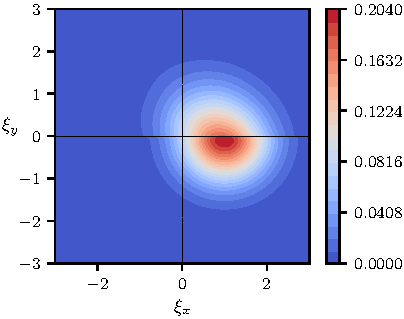
\includegraphics{{{distrib_f/kn0.1-boundary}}}
        \caption{возле пластины \(y=-0.499\)}
    	\label{fig:distrib-kn0.1:boundary}
    \end{subfigure}\\
    \begin{subfigure}[b]{\linewidth}
        \centering
        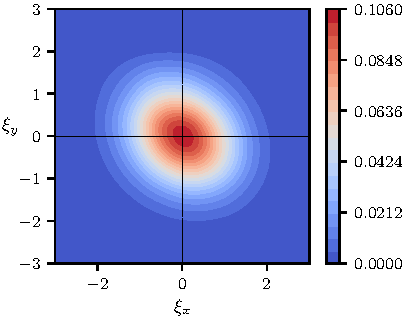
\includegraphics{{{distrib_f/kn0.1-center}}}
        \caption{возле оси симметрии \(y=-0.0082\)}
    	\label{fig:distrib-kn0.1:center}
    \end{subfigure}\\
    \caption{Функция распределения для \(\Kn=0.1\)}
    \label{fig:distrib-kn0.1}
\end{figure}
\begin{figure}
    \vspace{-24pt}
    \centering
    \begin{subfigure}[b]{\linewidth}
        \centering
        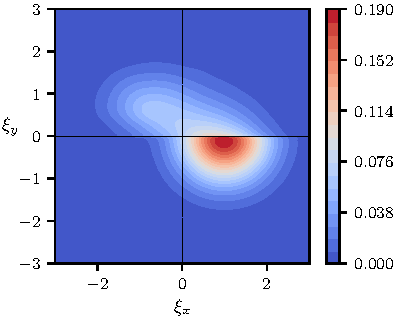
\includegraphics{{{distrib_f/kn1.0-boundary}}}
        \caption{возле пластины \(y=-0.493\)}
    	\label{fig:distrib-kn1.0:boundary}
    \end{subfigure}\\
    \begin{subfigure}[b]{\linewidth}
        \centering
        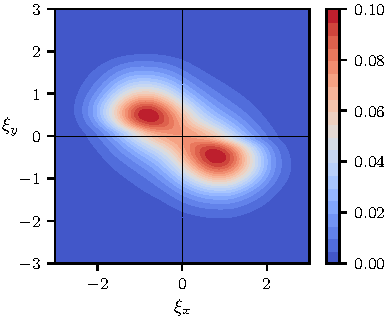
\includegraphics{{{distrib_f/kn1.0-center}}}
        \caption{возле оси симметрии \(y=-0.0083\)}
    	\label{fig:distrib-kn1.0:center}
    \end{subfigure}\\
    \caption{Функция распределения для \(\Kn=1\)}
    \label{fig:distrib-kn1.0}
\end{figure}
\begin{figure}
    \vspace{-24pt}
    \centering
    \begin{subfigure}[b]{\linewidth}
        \centering
        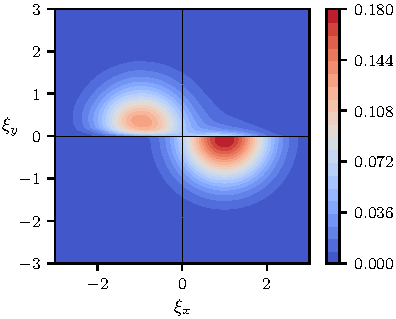
\includegraphics{{{distrib_f/kn10-boundary}}}
        \caption{возле пластины \(y=-0.492\)}
    	\label{fig:distrib-kn10:boundary}
    \end{subfigure}\\
    \begin{subfigure}[b]{\linewidth}
        \centering
        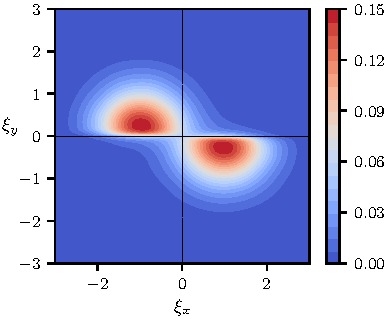
\includegraphics{{{distrib_f/kn10-center}}}
        \caption{возле оси симметрии \(y=-0.0083\)}
    	\label{fig:distrib-kn10:center}
    \end{subfigure}\\
    \caption{Функция распределения для \(\Kn=10\)}
    \label{fig:distrib-kn10}
\end{figure}

\section{Заключение}

На примере решения плоской задачи Куэтта можно провести сравнительный анализ применённых численных методов.
Для малых чисел Кнудсена, с точки зрения точности и экономичности, своё превосходство продемонстрировал
асимптотический анализ уравнения Больцмана.
Выводимые уравнения гидродинамического типа, совпадающие с уравнениями Навье--Стокса,
с соотвествующими граничными условиями скольжения позволяют получить
распределения макроскопических величин с погрешностью \(\mathcal{O}(\Kn^2)\).
Однако, в общем случае, во-первых, параметром разложения в приграничном вязкостном слое является \(\sqrt\Kn\),
а, во-вторых, асимптотический анализ в криволинейных координатах приводит к весьма громоздким выражениям~\cite{Sone2002}.
Кроме того, если вязкостный слой не гладок,
то способ конструирования асимптотического решения не очевиден~\cite{Aoki2014}.

При прямом численном решении уравнения Больцмана с помощью проекционного метода удалось добиться погрешности менее \(10^{-3}\)
для широкого диапазона внешних параметров: \(0.01 \le \Kn \le 100\) и \(0.1 \le \Delta{v} \le 5\).
Основная сложность получения высокоточного решения методом дискретных ординат
"--- это необходимость выбора соответствующей разностной сетки в скоростном пространстве
для обеспечения адекватной аппроксимации значительных колебаний функции распределения.
Высокая производительность проекционного метода связана с тем,
что дискретное скоростное пространство одинаково во всём объёме, занимаемом газом.
Для задач, где граничная поверхность имеет конечную кривизну,
приходится использовать равномерные скоростные сетки,
что значительно ухудшает аппроксимацию функции распределения в кнудсеновском слое.
Этой проблемы лишены методы статистического моделирования.
Метод DSMC, как и ожидалось, проявил свою универсальность,
однако не позволил получить достаточно точных результатов ввиду характерных статистических флуктуаций,
особенно для малых \(\Delta{v}\).
В настоящей работе прямое численное решение уравнения Больцмана в среднем потребовало на порядок больше времени,
чем статистическое моделирование, причём большего выигрыша DSMC добился для больших \(\Kn\).
Для малых \(\Kn\), как известно, требуются значительное увеличение времени моделирования столкновений.
С учётом вышесказанного, проекционный метод на неравномерных скоростных сетках можно рекомендовать
как прецизионный инструмент для решения уравнения Больцмана для любых чисел Кнудсена и Маха,
но для задач с простой прямоугольной геометрией.

\appendix
\appendixpage

\section{Функции Абрамовица}\label{sec:Abramowitz}

Семейство функций Абрамовица~\cite{Cercignani2000} имеют следующий вид:
\begin{equation}\label{eq:Abramowitz}
    \mathcal{T}_n(s) = \int_0^\infty t^n \exp\left(-t^2-\frac{s}{t}\right) \dd t,
    \quad s\ge0, \quad n \in \mathbb{Z}.
\end{equation}
Из очевидного соотношения \(\dd \mathcal{T}_n/\dd x = -\mathcal{T}_{n-1}\) следует, что
\[
    \lim_{s\to0} \frac{\dd^{n+1} \mathcal{T}_n(s)}{\dd s^{n+1}} = \infty.
\]
Таким образом, функции \(\mathcal{T}_n(s)\) неаналитичны ввиду особенности в точке \(x=0\),
поэтому не могут быть разложены непосредственно в ряд Тейлора.

Найдём, тем не менее, приближение \(\mathcal{T}_0(s)\) при малых \(s\):\footnote{
    В монографии К.~Черчиньяни <<Динамика разреженного газа>>~(2000)~\cite{Cercignani2000}
    допущена ошибка в форм.~(2.4.19).
}
\begin{gather}
    \mathcal{T}_0(s) = \int_0^1 \left(e^{-t^2}-1\right) e^{-\frac{s}{t}} \dd{t}
        + \int_1^\infty e^{-t^2} e^{-\frac{s}{t}} \dd{t}
        + \int_0^1 e^{-\frac{s}{t}} \dd{t} \notag\\
    = \int_0^1 \left(e^{-t^2}-1\right) \sum_{k=0}^2 \frac{(-s)^k}{k!t^k} \dd{t}
        + \int_1^\infty e^{-t^2} \sum_{k=0}^2 \frac{(-s)^k}{k!t^k} \dd{t}
        + s\int_s^\infty \frac{e^{-t}}{t^2} \dd{t} + o(s^2) \notag\\
    = \left(\frac{\sqrt\pi}2-1\right)
        + \frac{\gamma}2 s
        + (1-\sqrt\pi) \frac{s^2}2
        + e^{-s} - \int_s^\infty\frac{e^{-t}}{t} \dd{t} + o(s^2)  \notag\\
    = \frac{\sqrt\pi}2
        + s\ln{s} + \left(\frac{3\gamma}2 - 1\right) s
        - \sqrt\pi\frac{s^2}2 + o(s^2) \label{eq:Abramowitz0}
\end{gather}
Здесь используется интегральная показательная функция
\begin{equation}\label{eq:exp_integral}
    \mathrm{Ei}(s) = -\int_{-s}^\infty \frac{e^{-t}}{t} \dd{t}
        = \gamma + \ln|s| + \sum_{k=1}^{\infty} \frac{s^k}{kk!},
\end{equation}
где \(\gamma\) "--- постоянная Эйлера"--~Маскерони:
\begin{equation}\label{eq:euler-masceroni}
    \gamma = -\int_0^\infty e^{-t}\ln{t} \dd{t}
        = \int_0^1 \frac{1-e^{-t}}{t} \dd{t} - \int_1^\infty \frac{e^{-t}}{t} \dd{t}.
\end{equation}

Дальнейшее разложение в ряд приводит к следующим рекуррентным
соотношениям~\cite{Abramowitz1953,Abramowitz1972}:\footnote{
    В справочнике по специальным функциям М.~Абрамовица, И.~Стиган~(1979)~\cite{Abramowitz1972}
    см. форм.~(27.5.4).
}
\begin{gather}\label{eq:Abramowitz1-full}
    \mathcal{T}_1(s) = \frac12\sum_{k=0}^\infty ( a_k \ln{k} + b_k ) s^k, \\
    \begin{alignedat}{2}
        a_k &= \frac{-2a_{k-2}}{k(k-1)(k-2)}, &\quad b_k &= \frac{-2b_{k-2} - (3k^2-6k+2)a_k}{k(k-1)(k-2)}, \quad k>2, \\
        a_0 &= a_1 = 0, \quad a_2 = -1, &\quad b_0 &= 1, \quad b_1 = -\sqrt\pi, \quad b_2 = \frac32(1-\gamma).
    \end{alignedat} \notag
\end{gather}
В частности, дифференцируя~\eqref{eq:Abramowitz0}, получаем
\begin{equation}\label{eq:Abramowitz-1}
    \mathcal{T}_{-1}(s) = - \ln{s} - \frac{3\gamma}2 + \sqrt\pi s + O(s^2\ln{s}).
\end{equation}

\section{Численное решение задачи Куэтта для модели БКВ}\label{sec:numerical_bkw}

Решение задачи Куэтта в рамках линеаризованного уравнения БКВ
сводится к решению уравнения~\eqref{eq:bkw_g_equation}.
Основная сложность решения неоднородного интегрального уравнения Фредгольма второго рода для \(g(y)\)
"--- это логарифмические особенности ядра и первой производной свободного члена
[см.~\eqref{eq:Abramowitz0} и~\eqref{eq:Abramowitz-1}].
Как следствие, первая производная от \(g(y)\)
будет также иметь логарифмическую особенность на границе:\footnote{
    В работе Виллиса~(1962)~\cite{Willis1962} в форм. (2.14) допущено две опечатки.
    Правильный вариант: \( (dG/d\eta) \to G(0)J_{-1}(\eta)/2J_0(0) \to -\pi^{-\frac12}G(0)\ln(\eta)\).
}
\begin{equation}
    \frac{\dd{g}}{\dd{y}} = \frac1{k\sqrt\pi}\left[g\left(\frac12\right)-1\right]\ln\left(\frac12-y\right) + O(1).
\end{equation}

Метод решения подобных интегральных уравнений описан, например, в~\cite{Atkinson1997}
(см. главу 4.2) и основан на исключении из конечно-разностной аппроксимации
соответствующей сингулярности.
Поскольку свободный член в~\eqref{eq:bkw_g_equation} является приближённым решением для \(k\gg1\),
то непосредственное численное конечно-разностное решение уравнения~\eqref{eq:bkw_g_equation}
не вызывает сложностей для \(k\gtrsim1\). Для малых \(k\) решение~\eqref{eq:bkw_g_equation}
требует больших вычислительных затрат, однако уже для \(k \lesssim 0.05\) будет справедливо
асимптотическое решение~\eqref{eq:small_macro}, как минимум с точностью до 4 знаков.


\printbibliography

\end{document}
